\subsection{Rotina de Leitura dos Sensores}
\label{subsec:rotina_sensores}
% TODO:
% REALIZAR ANÁLISE DE FREQ. MÁXIMA DE OPERAÇÃO DOS ENCODERS VS BANDA DISPONIVEL NAS INTERRUPÇÕES RESPONSAVEIS PELA LEITURA DOS ENCODERS

Há duas interrupções associadas aos sinais provenientes dos \emph{Encoders} rotativos, uma para cada motor, cujo objetivo é medir a velocidade de rotação do eixo do motor ($\omega_{medido}$) bem como aplicar o filtro de \emph{Kalman} para uma melhor estimativa da mesma ($\hat{\omega}$). As interrupções são provocadas pelas bordas dos pulsos de ambos os canais, fazendo com que a resolução do sensor seja utilizada ao máximo, pois dessa maneira os sensores que possuem uma resolução de três pulsos por revolução (em cada canal, ver Figura \ref{fig:ilustracao_uma_revolucao}) consiga acionar doze (12) vezes a interrupção que irá computar o $\omega_{motor}$, passando assim a ser ter uma resolução equivalente à doze pulsos por revolução.\\

Para o cálculo do módulo da velocidade de rotação do eixo do motor faz-se uso da medição pelo período do sinal (conforme a Equação \ref{eq:omega_periodimetro}) com os seguintes parâmetros:

\begin{itemize}
    \item $N_{PR} = 12$. Pois são $12$ interrupções por canal (monitorando ambas as bordas de subida e descida de um dos canais);
    \item $T_{hf} = 1\mu{}s$. O contador de alta precisão do $ESP32$ possui, idealmente, uma resolução de $1\mu{}s$ \cite{esp}.
\end{itemize}

A escolha do método de leitura por periodímetro ao em vez do frequencímetro se deu devido assim ser possível a leitura imediata da velocidade, pois basta apenas uma interrupção para se ter uma medição e também devido a boa precisão da leitura para baixas velocidades, mesmo que isso piore para altas velocidades (como mostrado na Equação \ref{eq:erro_quantizacao_periodimetro}).

\begin{figure}[H]
    \centering
    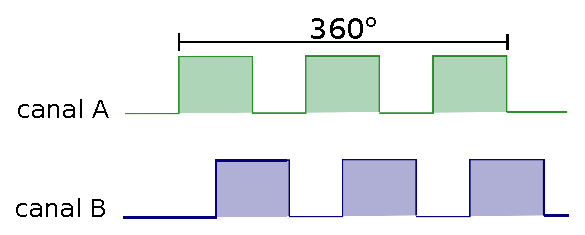
\includegraphics[width=0.5\textwidth]{figuras/ilustracoes/sinal_enquadratura_uma_revolucao.eps}
    \caption{Ilustração do sinal em quadratura em uma revolução completa do eixo do motor no sentido horário.}
    \label{fig:ilustracao_uma_revolucao}
\end{figure}

Já para se obter o sentido de rotação do motor, fez-se uso do padrão \emph{Gray Code} gerado pela diferença de fase entre os diferentes canais de um mesmo sensor. Uma maneira de fazer isso é ler os \emph{GPIO}'s associados aos canais do \emph{Encoder} e verificar o padrão em binário e inferir o sentido de rotação (conforme apresentado na \autoref{sec:encoders}). Porém esse procedimento apresentou uma alta taxa de erro na inferência do sentido para medias e altas velocidades. \\

A abordagem adotada aqui foi armazenar os dois \emph{bits}(sendo canal A bit mais significado) e concatenar/somar com os últimos dois \emph{bits} (da leitura anterior) deslocados em dois (equivalente à multiplicar por $2^2$ ou operar bit-a-bit: $bits_{anteriores} << 2$), criando assim um padrão com $4$ \emph{bits}, sendo os dois mais significados o padrão da leitura anterior e os dois menos significativos a leitura atual. Esse procedimento é ilustrado para uma rotação no sentido horário e no sentido anti-horário respectivamente nas Tabelas \ref{tab:tabela_gray_code_cw} e \ref{tab:tabela_gray_code_ccw}, dessa forma gera-se quatro($4$) padrões/códigos que caracterizam um tipo de rotação. Esse padrão de $4$\emph{bits} é armazenado de forma estática em um vetor(uma tabela de cola/ \emph{lookup table}) nas rotinas de ambos os motores, esse vetor mapeia o código binário em $1$, $-1$ ou zero para as combinações que não caracterizam um sentido de giro, o sinal do valor corresponde ao sentido horário ou anti-horário e depende do motor. Os vetores \emph{lookup table} para ambos os motores são apresentados  nas Tabela \ref{tab:lookup_table_motor_esquerdo} e \ref{tab:lookup_table_motor_direito}.

% Please add the following required packages to your document preamble:
% \usepackage{graphicx}
\begin{table}[H]
\centering
\resizebox{0.5\textwidth}{!}{%
\begin{tabular}{c|c|c|c|c}
\textbf{$A_{ant}$} & \textbf{$B_{ant}$} & \textbf{$A_{atual}$} & \textbf{$B_{atual}$} & \textbf{DEC} \\ \hline
0 & 0 & 1 & 0 & 2 \\
1 & 0 & 1 & 1 & 11 \\
1 & 1 & 0 & 1 & 13 \\
0 & 1 & 0 & 0 & 4
\end{tabular}%
}
\caption{Codificação de 4 \emph{bits} para a rotação no sentido horário.}
\label{tab:tabela_gray_code_cw}
\end{table}
% Please add the following required packages to your document preamble:
% \usepackage{graphicx}
\begin{table}[H]
\centering
\resizebox{0.5\textwidth}{!}{%
\begin{tabular}{c|c|c|c|c}
\textbf{$A_{ant}$} & \textbf{$B_{ant}$} & \textbf{$A_{atual}$} & \textbf{$B_{atual}$} & \textbf{DEC} \\ \hline
0 & 0 & 0 & 1 & 1  \\
0 & 1 & 1 & 1 & 7  \\
1 & 1 & 1 & 0 & 14 \\
1 & 0 & 0 & 0 & 8 
\end{tabular}%
}
\caption{Codificação de 4 \emph{bits} para a rotação no sentido anti-horário.}
\label{tab:tabela_gray_code_ccw}
\end{table}
% Please add the following required packages to your document preamble:
% \usepackage{graphicx}
\begin{table}[H]
\centering
\resizebox{0.8\textwidth}{!}{%
\begin{tabular}{c|ccccllllllllllll}
\textbf{Índice} & 0 & 1  & 2 & 3 & 4 & 5 & 6 & 7  & 8  & 9 & 10 & 11 & 12 & 13 & 14 & 15 \\ \hline
\textbf{Valor}  & 0 & -1 & 1 & 0 & 1 & 0 & 0 & -1 & -1 & 0 & 0  & 1  & 0  & 1  & -1 & 0 
\end{tabular}%
}
\caption{\emph{Lookup table} para o motor esquerdo.}
\label{tab:lookup_table_motor_esquerdo}
\end{table}
% Please add the following required packages to your document preamble:
% \usepackage{graphicx}
\begin{table}[H]
\centering
\resizebox{0.8\textwidth}{!}{%
\begin{tabular}{c|ccccllllllllllll}
\textbf{Índice} & 0 & 1  & 2 & 3 & 4 & 5 & 6 & 7  & 8  & 9 & 10 & 11 & 12 & 13 & 14 & 15 \\ \hline
\textbf{Valor}  & 0 & 1 & -1 & 0 & -1 & 0 & 0 & 1 & 1 & 0 & 0  & -1  & 0  & -1  & 1 & 0 
\end{tabular}%
}
\caption{\emph{Lookup table} para o motor direito.}
\label{tab:lookup_table_motor_direito}
\end{table}

Com a \emph{lookup table} e o módulo da velocidade é possível calcular a velocidade de rotação da seguinte forma:

\begin{equation}
    \omega_{medido} = \frac{2\pi}{N_{PR}\Delta{t}}table[code]
\end{equation}

Sendo,

\begin{equation*}
    \Delta{t} = nT_{hf}
\end{equation*}

Uma vez calculado o $\omega_{medido}$, calcula-se em 
seguida a melhor estimativa para $\omega$ ($\hat{\omega}$) 
utilizando-se o filtro de \emph{Kalman} (conforme apresentado na \autoref{sec:kalman}). 
Para isso é considerado que o sistema $\omega(t)$ possui um comportamento de primeira ordem 
(conforme Equação \ref{eq:motor_transf_func}), fazendo com que as variáveis do filtro sejam:

\begin{equation*}
\begin{cases}
    \textbf{x}_k = \left[ \omega_k \right]\\
    \textbf{z}_k = x_k = [\omega_k]\\
    \textbf{F}_k = [1]\\
    \textbf{H}_k = [1]
\end{cases}
\end{equation*}

Modelo da \textbf{medição}:
\begin{align*}
z_k = \omega_{medido}
\end{align*}

Com isso a etapa de \textbf{predição} do filtro torna-se:
% MUDAR O SIMBOLO QUE FAZ REFERENCIA À ENTRADA (u) DE ENTRADA
\begin{align*}
    \check{\omega}_{k|k-1} &= \hat{\omega}_{k-1} + (u_k.K_m - \hat{\omega}_{k-1})\left( 1 - e^{-\Delta{t}/T_m} \right)\\
    \check{P}_{k|k-1} &= \hat{P}_{k-1} + Q_k
\end{align*}

Sendo $u_k$ o sinal de controle no instante $k$.\\

E a etapa de atualização \textbf{Atualização} é:

\begin{align*}
K_k &= \check{P}_k \left( \check{P}_k + R_k \right)^{-1} = \frac{\check{P}_k}{\check{P}_k + R_k}\\
\hat{\omega}_k &= \check{\omega}_k + K_k \left( \omega_{k_{medido}} - \check{\omega}_k \right)\\
\hat{P}_k &= \left( 1 - K_k \right) \check{P}_k
\end{align*}

Os parâmetros do filtro foram sintonizados experimentalmente, sendo eles:

\begin{itemize}
    \item $Q = 10$;
    \item $R = 1200$, notou-se pouca variação nesse valor da variância da medição (o valor foi obtido calculando-se a variância da resposta da planta/motor em regime permanente).
    \item $P_0 = 60$, valor inicial da incerteza da melhor estimativa.
\end{itemize}

Foram utilizados estruturas do tipo fila (\emph{Queue} de tamanho 1, para não causar atrasos extras) para enviar e receber estruturas de dados entre as interrupções dos sensores e as demais rotinas em execução no ESP32. Dessa maneira foi possível evitar o uso de variáveis globais e permitiu a troca de informação com a rotina de controle que fica em execução em um núcleo diferente do microcontrolador. O fila de saída contém a estimativa da velocidade e a fila de entrada contém os parâmetros do filtro, bem como o último sinal de controle. Um pseudo código ilustrando a rotina de leitura dos sensores é apresentado a seguir:

\begin{algorithm}
\caption{Rotina de Leitura dos Sensores}
\label{alg:rotina_leitura_sensores}
\begin{algorithmic}[1]
  \State $lookup\_table \gets $ \{0, 1, -1, 0, 0, 0, 0, 1, 0, 0, 0, -1, 0, 1, -1, 0\}

  % atualiza o codigo
  \State $code \gets \left(code \ll 2\right) + \left(\left(READ\_GPIO(CANAL\_A)\ll1\right)+READ\_GPIO(CANAL\_B)\right)$

  \State $t_1 \gets get\_time()$ \Comment{Obtém o tempo atual em segundos.}
  
  \State $\Delta{t} \gets  t_1 - t_0$
  
  \State $t_0 \gets t_1$ \Comment{Atualiza a referência de tempo anterior $t_0$}
  
  \State $\omega_{medido} \gets \frac{2\pi}{N_{PR}*\Delta{t}}$ * $lookup\_table[code]$
  
  \If{ $queue\_input.empty()$ \textbf{E} nunca recebeu} \Comment{Verifica se tem os dados para usar o filtro.}
    \State $queue\_output \gets \omega_{medido}$  \Comment{Coloca o $\omega_{medido}$ na fila de saída e encerra a rotina.}
    \State return;
  \EndIf
  
  \Comment{Caso tenha novos dados (fila de entrada não vazia) atualizar os dados presentes na rotina. Se não usar os dados anteriores.}
  \State $\omega_{ss}$,$\tau$ $\gets  queue\_input$

%   //predição
  \Comment{Etapa de predição.}
  \State $\check{\omega} \gets \omega_{medido}$ + $( \omega_{ss} - \omega_{medido} ) * (1 - exp(-\Delta{t}/\tau))$
  \State $\check{P} \gets \hat{P} + Q$


%   //atualização
  \Comment{Etapa de atualização.}
  \State $K_{gain} \gets \check{P} / (\check{P} + R)$
  \State $\hat{\omega} \gets \check{\omega}$ + $K_{gain} * (\omega_{medido} - \check{\omega})$
  \State $\hat{P} \gets (1 - K_{gain}) * \check{P}$ 
  
  \State $queue\_output \gets \hat{\omega}$
\end{algorithmic}
\end{algorithm}
